%\newcommand{\CLASSINPUTbottomtextmargin}{20mm}
\documentclass[conference,a4paper]{IEEEtran}

%\usepackage{showframe}
\usepackage{comment}
\usepackage[subpreambles=true]{standalone}
\usepackage{graphicx}
\usepackage{hyperref} % Use before cleveref
\usepackage{cleveref}
\usepackage{footnote}
\usepackage{url}
\usepackage[inline]{enumitem}

\newcommand{\citeneeded}{\textbf{{[}citation needed{]}}}
\newcommand{\TC}{tangled commit}
\newcommand{\GCR}{Gerrit Code Review}
\newcommand{\Ep}{Epicea}
\newcommand{\Gr}{Griotte}
\newcommand{\code}[1]{\texttt{#1}}
\newcommand{\todo}[1]{\textbf{\textcolor{red}{{[}TODO: #1{]}}}}

\title{\Gr{}: Improving Code Review\\with Fine-Grained IDE Events}

\author{\IEEEauthorblockN{Skip~Lentz}\IEEEauthorblockA{EEMCS\\Delft
    University of Technology} \and
  \IEEEauthorblockN{Mart\'{i}n~Dias}\IEEEauthorblockA{RMoD\\INRIA
    Lille-Nord Europe}}

\begin{document}
\maketitle{}
\begin{abstract}
  Code review is a difficult process because:
  \begin{enumerate*}[label=(\arabic*)]
  \item developers often create \textit{tangled commits},
  \item a change may be scattered across many different parts of a
    project,
  \item many changes are shadowed,
  \item commit messages can be inaccurate or wrong and
  \end{enumerate*}

  This work aims to propose a solution to these problems by exploiting
  the information provided by fine-grained IDE events.

  To put this solution in practice, we will develop a code review tool
  named \textit{\Gr} in the \textit{Pharo} environment.
\end{abstract}
\begin{IEEEkeywords}
  code review, fine-grained IDE events, \Ep, \Gr, Pharo
\end{IEEEkeywords}

\section{Problem Description}
\label{sec:problem-description}
Modern Code Review (MCR) is an important mechanism for quality
assurance in software development: it provides feedback and helps to
avoid introducing bugs. However, it is a difficult task for a reviewer
to perform because:

\paragraph{Tangled commit}

A \TC{} is a commit which is the result of multiple, mutually
unrelated changes. For example, a commit could consist of a
refactoring, some formatting changes, and a bug fix.

The process of understanding a change is difficult on its own. In the
case of a tangled commit, the reviewer in addition has to understand
several unrelated changes at the same time.

Herzig \& Zeller found in a study of five open-source Java projects,
that up to 15\% of all bug fixes consist of multiple unrelated
changes\cite{Herz11a}.

\paragraph{Line-based view}

Commits may have changes scattered across many different parts of a
project. For example, a method rename impacts all method
references. However, even though the changes belong together, they are
not shown together within the changes browser of the code review
tool. For this reason, we say that these review tools are
\textit{line-based}.

Thus, the reviewer has to analyze the changes line-by-line to conclude
that it was a refactoring, which is not a trivial task.

\paragraph{Shadowed changes}

Negara \textit{et al.} found that 37\% of changes are
\textit{shadowed}, \textit{i.e.} overridden by subsequent changes in
the same line, file and commit\cite{Nega12a}. This can be important
information for the reviewer to find out how the developer arrived at
their solution.

\paragraph{Wrong or lack of commit descriptions}

Commit descriptions can help the reviewer in understanding the reason
of a change. Without the description, the reason for a change is
lost. Furthermore, a wrong description has the potential to mislead
the reviewer.

Commit messages are often inaccurate or wrong\citeneeded{}.

\section{Proposed Solution}
\label{sec:proposed-solution}
This section aims to propose several solution approaches which use the
information provided by \textit{fine-grained IDE events}. First, we
will explain what fine-grained IDE events are. Then we will discuss
how they might be used to solve the problems mentioned in
\Cref{sec:problem-description}.

\subsection{Fine-grained IDE events}
\label{sec:fine-grained-ide}

Normally when a developer works on a feature or fixes a bug, the
changes are recorded at the point of commit. The actions the developer
has performed to get to that state are lost, and are collapsed into
one change. These intermediate actions are known as
\textit{fine-grained IDE events} --- in contrast with the
\textit{coarse-grained} changes one might find in a VCS commit.

An example of fine-grained IDE events can be found in
\Cref{fig:ide-event-class-model}. The events described in the diagram
are recorded and stored as the developer is working in the IDE.
\begin{figure}[h]
  \centering
  \resizebox{!}{0.3\textheight}{%
    \documentclass[crop]{standalone}

\usepackage{tikz}
\usetikzlibrary{trees,calc}
\begin{document}

\tikzstyle{every node}=[draw=black,thick,anchor=west]
\tikzstyle{grayed node}=[draw=black!60,text=black!60,dashed]

%\small
\sffamily

\begin{tikzpicture}[%
    grow via three points={
        one child at (0.8,-0.7) and two children at (0.8,-0.7) and (0.8,-1.4)
    },
    edge from parent path={
        ($(\tikzparentnode\tikzparentanchor)+(.4cm,0pt)$) |- (\tikzchildnode\tikzchildanchor)
    },
    growth parent anchor=west,
    parent anchor=south west]
  \node {IDE event}
    child { node {code change}
    child { node {class change}
      child { node {class addition}}
      child { node {class modification}}
      child { node {class removal}}
      child { node {class comment}}
    }
    child [missing] {}
    child [missing] {}
    child [missing] {}
    child [missing] {}
    child { node {method change}
      child { node {method addition}}
      child { node {method modification}}
      child { node {method removal}}
    }
    child [missing] {}
    child [missing] {}
    child [missing] {}
    child [missing] {}
    child [missing] {}
    child [missing] {}
    }
    child [missing] {}
    child [missing] {}
    child [missing] {}
    child [missing] {}
    child [missing] {}
    child [missing] {}
    child [missing] {}
    child [missing] {}
    child [missing] {}
    child { node {test unit run}}
    child { node {versioning operation}
      child { node {version save}}
      child { node {version load}}
    }
    child [missing] {}
    child [missing] {}
    child { node {refactoring run}}
    child { node {IDE session}}
    child { node {undo/redo}}
    child [missing] {};
\end{tikzpicture}

\end{document}

%\MC & save, load \\

%%% Local Variables:
%%% mode: latex
%%% TeX-master: t
%%% End:

  }
  \caption{A minimized class diagram of a model for fine-grained IDE
    events}
  \label{fig:ide-event-class-model}
\end{figure}

Fine-grained IDE events supply significant additional information
compared to the changes found in a typical VCS repository, as many of
the fine-grained IDE events are shadowed\cite{Nega12a}.

\subsection{Code review using fine-grained IDE events}
\label{sec:code-review-using-1}

There are several approaches where fine-grained IDE events are useful
in the context of code review. Each approach corresponds to one or
more of the problems listed in \Cref{sec:problem-description}.

\paragraph{Displaying fine-grained history}

A solution approach is to display the information to the
reviewer. This allows the reviewer to see how a developer evolved to
the submitted change. This solves problem c) in that it shows extra
information which is typically shadowed by other changes.

\paragraph{Grouping changes}

An approach to solve problems a) and b) % TODO: use references
is to group changes. A group of changes consists of one or more code
changes which are mutually related, along with a descriptive label
(e.g. a refactoring of method name \code{foo} to \code{bar}). By
grouping the changes, we change the perspective from a
\textit{line}-based review tool to a \textit{change}-based review
tool.

Work has been done in this area: Tao and Kim\cite{Tao15a} have
explored grouping (referred to as \textit{partitioning}) tangled
commits (\textit{composite changes}) in the context of code
review. However, they partitioned changes using only the information
available from the VCS.

Dias \textit{et al.}\cite{Dias15a} have done work on untangling
commits using fine-grained IDE events, with good results; namely 88\%
accuracy in determining whether two code changes belong together.

We aim to combine both approaches --- groups in the context of review
and grouping using fine-grained IDE events \todo{Which terminology
  should be used: ``groups'' or ``untangled commits''}.

\paragraph{Generating commit descriptions}

\todo{Maybe not?}

\section{Implementation: Griotte}
\label{sec:impl-griotte}

To put the solution approaches mentioned in
\Cref{sec:proposed-solution} in practice, we will develop a code
review tool named \textit{Griotte}. The core concept in the
architecture of Griotte is the usage of existing services which
provide code review features (\textit{e.g.} \textit{GitHub} or
\textit{Gerrit}). See \Cref{fig:diagram} for a simplified diagram of
the architecture.
\begin{figure}[t]
  \centering{\resizebox{\linewidth}{!}{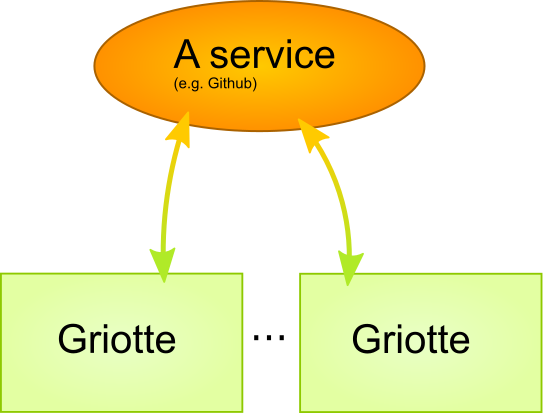
\includegraphics{idea.png}}}
  \caption{Simplified architecture diagram of Griotte}
  \label{fig:diagram}
\end{figure}

Griotte will be implemented in the \textit{Pharo}
environment\cite{Blac09a}\footnote{Pharo: \url{http://pharo.org}}.
Furthermore, we will use \textit{Epicea}\cite{Dias13a} to monitor and
access fine-grained IDE events.

First, a brief description of Epicea will be given. Afterwards, we
will discuss the implementation of Griotte in more detail.

\subsection{Epicea}
\label{sec:epicea}

\Ep\ is a Pharo project providing a model for first-class code changes
and related IDE tools. \Ep\ records IDE events during development,
allowing us to analyze a more fine-grained history of the
codebase. This is in contrast with the code change information
available from a VCS repository, which is much more coarse-grained.

The model of \Ep\ is described by \Cref{fig:ide-event-class-model}. It
can be divided into \textit{low-level} and \textit{high-level} IDE
events.

Low-level IDE events are code changes --- additions, deletions or
modifications --- of program components such as classes or
methods. Examples are a method modification, a class addition, etc.

Secondly, \Ep\ records IDE events such as a test run (and its
outcome), refactorings, and loading a version from the VCS. These are
known as high-level IDE events.

\Ep\ records this data by means of the \textit{\Ep\ Monitor}, which
listens to events in Pharo as they happen, and converts them to the
first-class code change model objects described in
\Cref{fig:ide-event-class-model}. These objects are then stored and
persisted in a log.

\subsection{Griotte}
\label{sec:griotte}

An important part of Griotte is the usage of existing services which
provide code review features. Examples of these services are
\textit{GitHub} or \textit{Gerrit}. The extra information provided by
the fine-grained IDE events will be stored as metadata. For example,
in \code{git}-based repository services, we can use
\code{git-notes}\footnote{Documentation:
  \url{http://git-scm.com/docs/git-notes}} to store metadata on
commits. The Griotte client within Pharo will then be used for the
features using the fine-grained IDE events.

A good advantage is that this makes it possible to use Griotte in
parallel with other workflows, since the metadata is stored in a
manner transparent to common workflows.

Furthermore, we don't need to maintain our own servers if we choose to
use GitHub or similar services. The maintenance of both server-side
code and the servers will be done by others.

A disadvantage is that we need to sacrifice some of our own
flexibility, and rely on the flexibility of the API's of external
services like GitHub. In a research project this might seem less
ideal, as one would like to be free to explore different
options.

\begin{comment}
\section{Forming Groups using First-Class Code Changes}
\label{sec:code-review-using}
There are different strategies we can employ to form groups of code
changes. In the simplest sense, they can be formed automatically or
manually. In this section we discuss which strategy --- automatic or
manual --- is the right one for various kinds of groups.

\subsection{Automatically forming groups}
\label{sec:autom-form-groups}
The automatic approach is likely the most suitable for code changes
done by a refactoring. Since refactorings are provided with rich
information in the Epicea model, forming this code change as a group
and creating a descriptive label should be straightforward.

Another approach is comparing the \textit{abstract syntax tree}\ (AST)
to detect whether or not the code change entails a change of behavior
in the program. While the detection of this is straightforward,
creating a descriptive label is less so. For example, both the
addition of a comment and a formatting in the body of a method cause
no change in the AST. Thus, in this case, the labels of the groups
become less descriptive. However, even a non-descriptive label such as
``No change in behavior'' assists the reviewer in understanding the
code more than there being no label at all.

We foresee a challenge in this approach; namely that many changes are
shadowed or undone and thus do not reach the
VCS\cite{Nega12a}. Detecting this is not trivial, but necessary to
reduce the unneeded groups in the output.

\subsection{Manually forming groups}
\label{sec:manu-form-groups}
When groups are formed manually, we have the benefit of being able to
create a very precise label for the group. An obvious downside is that
this requires us to count on the assistance of the developer. A
separate tool for this could therefore prove useful.

An example of such a tool is the \textit{\Ep\ Task
  Clusterer}\cite{Dias15a}, which provides the developer with an
intuitive user interface to group ``tasks''. In this context, a task
refers to the resulting code of resolving an issue or bug-report.

\section{Implementation}
\label{sec:implementation}
We aim to implement a code review tool named \textit{\Gr} for Pharo
which employs the concept of groups. This section aims to present the
implementation of the tool. An important part of the tool is that it
leverages existing services providing code review features such as
\textit{GitHub} or \textit{Gerrit}. See \Cref{fig:diagram} for a
simplified diagram of the architecture.

\subsection{Leveraging existing services}
\label{sec:lever-exist-serv}
A key part of our implementation will be the use of existing
services. We discuss the advantages and disadvantages, and how this
approach is to be implemented.

An advantage is that this allows us to alleviate ourselves from part
of the maintenance of the code review tool. This includes both server
maintenance and server-side code maintenance. Furthermore, we get
security and additional functionality for free.

A disadvantage is that we need to sacrifice some of our own
flexibility, and rely on the flexibility of the API's of external
services like GitHub. In a research project this might seem less
ideal, as one would like to be free to explore different
options. However, we feel that we have found the middle way between a
pragmatic solution and a more research oriented solution.

The idea is that the special features which use the concept of groups
are to be accessible only client-side, i.e. from within Pharo. The
information necessary for the groups can be stored as metadata on the
external service. For example, in the case of git-based services such
as GitHub or Gerrit, we can use the
\code{git-notes}\footnote{Documentation:
  \url{http://git-scm.com/docs/git-notes}} model to store metadata on
commits.
\end{comment}

\section{Conclusion}
\label{sec:conclusion}

To conclude and summarize, we presented the following difficulties
with code review:
\begin{enumerate}[label=(\arabic*)]
\item Developers often create \textit{tangled commits}. Reviewers have
  to understand multiple unrelated changes at the same time.
\item Code review tools are line-based. Commits may touch many
  different parts of a project, and the reviewer has to analyze each
  change line-by-line even if they are related to the same change.
\item Many changes are shadowed, which can be important information
  for the reviewer.
\item Commit messages can be inaccurate or wrong, which misleads the
  reviewer or does not provide enough information.
\end{enumerate}

We proposed several solution approaches which use fine-grained IDE
events in the context of code review:
\begin{enumerate}[label=(\arabic*)]
\item Display fine-grained history to the reviewer, to provide extra
  information if it's needed.
\item Group mutually related changes together using the fine-grained
  IDE events as input.
\item Generate accurate commit descriptions using the information
  provided by fine-grained IDE events.
\end{enumerate}

Furthermore, we presented our proposal for an implementation of a code
review tool named Griotte which \begin{enumerate*}[label=(\arabic*)]
\item uses these approaches, \item is implemented in the Pharo
  environment and \item uses Epicea as a source for fine-grained IDE
  events \end{enumerate*}. A key idea of our implementation is the use
of existing external services such as GitHub and Gerrit. We discussed
the benefits and limitations of this approach.

\bibliographystyle{IEEEtran}
\bibliography{IEEEabrv,rmod,others}
\end{document}

%%% Local Variables:
%%% mode: latex
%%% TeX-master: t
%%% End:
